\chapter{Modelado del Problema}

En este capítulo se detalla cómo se ha construido el entorno virtual sobre el que operarán los algoritmos de búsqueda. El objetivo principal es transformar un espacio geográfico real (el parque de la Casa de Campo en Madrid) en un modelo matemático y probabilístico que los drones puedan entender y procesar de forma eficiente.

\section{Generación del Espacio de Búsqueda}

El problema de Búsqueda en Tiempo Mínimo (MTS) requiere definir primero la región espacial operativa. Este espacio continuo bidimensional se delimita y recorta para centrar los esfuerzos computacionales en la zona de interés. En el framework SAREnv, la región inicial de búsqueda se puede definir mediante dos metodologías:

\begin{enumerate}
    \item \textbf{Generación Radial por Punto Visto por Última Vez (PLS/LKP):} Se especifica un punto de coordenadas geográficas origen $(\text{Latitud}, \text{Longitud})$ correspondiente a la última posición conocida de la persona extraviada. Para evitar descargas infinitas de datos geográficos, el sistema utiliza tablas estadísticas internas basadas en el comportamiento histórico de personas perdidas (\textit{Lost Person Behavior} - LPB). Cruzando el tipo de topografía (llano, montañoso) y el clima (seco, templado), se selecciona el radio máximo estadístico de dispersión (talla extrema o \textit{xlarge}). Por ejemplo, para un relieve llano y clima templado, el radio máximo considerado es $r = 9.9$~km. Con este radio, se genera un círculo que delimita el espacio de búsqueda.
    \item \textbf{Generación Basada en Polígono Vectorial Personalizado:} Se define un polígono cerrado a medida mediante un conjunto de vértices geográficos. Usando la librería matemática \texttt{shapely.geometry.Polygon}, se crea una frontera geométrica estricta. Esta aproximación es ideal para recintos cerrados o parques urbanos delimitados, como el parque de la Casa de Campo de Madrid, ya que evita descargar zonas adyacentes irrelevantes (carreteras circundantes o zonas residenciales).
\end{enumerate}

Una vez definida la región geométrica, el sistema se conecta a la API de OpenStreetMap (OSM) mediante la librería de Python \texttt{osmnx} para descargar los datos vectoriales. Las geometrías resultantes se recortan aplicando la intersección geométrica:
\begin{equation}
    \mathcal{G}_{\text{final}} = \mathcal{G}_{\text{OSM}} \cap \mathcal{P}_{\text{búsqueda}}
\end{equation}
donde $\mathcal{G}_{\text{OSM}}$ son las características geográficas descargadas en bruto y $\mathcal{P}_{\text{búsqueda}}$ es el polígono del escenario del usuario. Esto descarta cualquier información fuera del lienzo de simulación.

\section{Proceso de Sectorización (Discretización)}

Los algoritmos de planificación de rutas en cuadrículas no pueden procesar un mapa geométrico continuo; requieren una representación discreta. Para ello, el espacio geográfico se sectoriza proyectándolo en una matriz bidimensional (rejilla o \textit{grid} de Numpy).

La resolución del mapa discreto se controla a través del parámetro fundamental $meter\_per\_bin$ (denotado como $\delta$), que establece cuántos metros reales mide cada lado de una celda de la cuadrícula. Para este trabajo, se ha seleccionado $\delta = 10$, lo que implica que cada celda o sector representa un área física real de $10 \times 10$ metros ($100~\text{m}^2$).

El framework calcula las dimensiones de la matriz de la siguiente manera. Sean $(x_{\min}, y_{\min})$ y $(x_{\max}, y_{\max})$ los límites coordenados proyectados (Bounds) del polígono de búsqueda, y $b$ el valor del margen de seguridad o \textit{buffer}. El número de celdas en el eje de abscisas ($N_x$) y ordenadas ($N_y$) se determina mediante:
\begin{equation}
    N_x = \left\lfloor \frac{|x_{\max} - x_{\min} + 2b|}{\delta} \right\rfloor
\end{equation}
\begin{equation}
    N_y = \left\lfloor \frac{|y_{\max} - y_{\min} + 2b|}{\delta} \right\rfloor
\end{equation}
donde $\lfloor \cdot \rfloor$ representa la función piso. El escenario discretizado completo de la Casa de Campo queda modelado por una matriz de $458 \times 481$ celdas, abarcando una superficie total de aproximadamente $12.75~\text{km}^2$. Cada celda de coordenadas discretas $(i, j)$ se asocia unívocamente a una zona física del parque.

\section{Fusión Probabilística Multicapa (SAREnv)}

Para que los drones puedan tomar decisiones orientadas a la optimización de la probabilidad, el espacio discreto debe asociarse a una distribución de probabilidad espacial inicial, conocida como Mapa de Creencias Inicial $b(v^0)$ o matriz de Probabilidad de Área (POA). El modelado probabilístico de SAREnv se construye en dos fases: un modelado continuo a nivel vectorial y una proyección discreta a nivel de rejilla.

\subsection{Modelado Continuo a Nivel Vectorial}

El parque de la Casa de Campo se representa mediante un conjunto de características geográficas discretas $\mathcal{F} = \{f_1, f_2, \dots, f_M\}$ extraídas de OpenStreetMap. Cada elemento geográfico $f \in \mathcal{F}$ posee un tipo $\tau = T(f)$ (por ejemplo, bosque, sendero o río). La probabilidad de que la persona extraviada se encuentre en una característica concreta depende de dos factores independientes: la tipología de la característica y su distancia al Punto de Planificación Inicial (IPP).

\begin{enumerate}
    \item \textbf{Peso Basado en la Tipología ($\omega_{\text{type}}$):} Define la verosimilitud de presencia según el perfil del sujeto y la naturaleza del terreno:
    \begin{equation}
        \omega_{\text{type}}(f) = P_{\text{type}}(T(f))
    \end{equation}
    donde $P_{\text{type}}$ es la probabilidad histórica asociada al tipo de característica $T(f)$ obtenida de las bases de datos de rescate (ISRID) \cite{koester2008lost, romero2018manual}.
    \item \textbf{Peso Basado en la Distancia Espacial ($\omega_{\text{spatial}}$):} Modela la dispersión radial de la víctima desde el IPP. El paper de SAREnv demuestra empíricamente que la distancia recorrida $d$ se ajusta óptimamente a una distribución log-normal (con un error RMSE de 1.76~km frente a los 6.83~km de una distribución normal):
    \begin{equation}
        \omega_{\text{spatial}}(f) \sim \text{LN}(d; \mu_{\text{LPB}}, \sigma_{\text{LPB}})
    \end{equation}
    donde $\mu_{\text{LPB}}$ y $\sigma_{\text{LPB}}$ son los parámetros de escala y forma ajustados para el clima templado y terreno llano.
\end{enumerate}

Asumiendo la independencia estadística entre la tipología y la localización espacial, la puntuación de verosimilitud combinada $S(f)$ para una característica $f$ se calcula como el producto de ambos pesos:
\begin{equation}
    S(f) = \omega_{\text{type}}(f) \cdot \omega_{\text{spatial}}(f)
\end{equation}

Finalmente, la Probabilidad de Área ($POA$) normalizada para cada característica vectorial $f_i$ se obtiene al dividir su puntuación por la suma de las puntuaciones de todas las características presentes en el dominio de búsqueda:
\begin{equation}
    POA(f_i) = \frac{S(f_i)}{\sum_{j=1}^{M} S(f_j)}
\end{equation}

\subsection{Proyección y Fusión a Nivel de Rejilla (Rasterización)}

Para su procesamiento autónomo por la flota de drones, los datos vectoriales y sus probabilidades asociadas se proyectan sobre el espacio discretizado de celdas $(i, j)$ de resolución $\delta = 10\text{ m}$.

Las características se clasifican en capas semánticas principales:
\begin{itemize}
    \item \textbf{Estructuras:} Edificios y refugios (\textit{tags}: \texttt{building}, \texttt{man\_made}).
    \item \textbf{Vías terrestres:} Caminos y senderos (\textit{tags}: \texttt{highway}, \texttt{track}).
    \item \textbf{Recursos hídricos:} Ríos y lagos (\textit{tags}: \texttt{waterway}, \texttt{natural:water}).
    \item \textbf{Zonas naturales:} Bosques y prados (\textit{tags}: \texttt{natural:wood}, \texttt{natural:scrub}).
\end{itemize}

A diferencia del diseño inicial de SAREnv, que utilizaba un operador de máximo en cada celda para evitar acumulaciones de probabilidad, en este trabajo se ha modificado la lógica de combinación para implementar una \textbf{suma ponderada y posterior normalización global}. 

El artículo original de SAREnv \cite{drones9090628} señala explícitamente como una limitación del operador de máximo el hecho de no considerar el efecto acumulativo cuando convergen múltiples características favorables en un mismo punto, lo que puede infravalorar zonas ricas en características (\textit{feature-rich zones}), tales como la confluencia de un sendero forestal con el acceso a una estructura.

Para resolver esta limitación, el proceso de fusión se formula en los siguientes pasos:
\begin{enumerate}
    \item \textbf{Rasterización de capas binarias:} Para cada capa $k$, se genera una matriz binaria $\mathbf{M}_k(i, j) \in \{0, 1\}$ indicando la presencia espacial del elemento.
    \item \textbf{Suma Ponderada Multicapa:}
    \begin{equation}
        \mathbf{POA}_{\text{unnorm}}(i, j) = \sum_{k} \mathbf{M}_k(i, j) \cdot \alpha_k
    \end{equation}
    donde $\alpha_k$ es el peso asignado a la capa $k$ según el perfil de búsqueda.
    \item \textbf{Normalización Global:}
    \begin{equation}
        \mathbf{POA}_{\text{norm}}(i, j) = \frac{\mathbf{POA}_{\text{unnorm}}(i, j)}{\sum_{u=1}^{N_y} \sum_{v=1}^{N_x} \mathbf{POA}_{\text{unnorm}}(u, v)}
    \end{equation}
\end{enumerate}

Debido a que la topología de OpenStreetMap genera capas de suelo (bosque, prados) geográficamente disjuntas que no se solapan entre sí, los únicos solapamientos se producen por elementos lineales (caminos) e infraestructuras sobre dichos fondos. Por tanto, la suma no genera un mapa diluido, sino que preserva los picos de los caminos y eleva de forma realista la importancia de sus intersecciones.

\section{Filtro Físico de Restricciones No Transitables y Búsqueda Coordinada}

En un entorno real de búsqueda terrestre, existen zonas donde la víctima no puede encontrarse de forma transitable a pie o donde los sensores aerotransportados del dron resultan inútiles, tales como el interior de masas de agua profunda (lagos y estanques principales) o el interior de edificaciones urbanas cerradas.

Para dotar al mapa de calor de coherencia operativa estricta, el sistema aplica un filtro de restricciones duras mediante indexación espacial jerárquica con árboles R-Tree (\texttt{sindex}). Para cada celda $(i, j)$ que intersecta con un polígono de masa de agua o edificio no transitable $\mathcal{G}_{\text{restringido}}$, su probabilidad se anula estrictamente:
\begin{equation}
    b(v^0)(i, j) = \begin{cases}
        0.0 & \text{si } (i, j) \cap \mathcal{G}_{\text{restringido}} \neq \emptyset \\
        \mathbf{POA}_{\text{norm}}(i, j) & \text{en otro caso}
    \end{cases}
\end{equation}
Tras la aplicación de la máscara, la matriz se renormaliza globalmente, asegurando que $\sum_{i,j} b(v^0)(i,j) = 1.0$.

\subsection{Justificación Operativa: La Búsqueda Coordinada en el Perfil Autista}

Un caso de estudio fundamental que justifica la necesidad de este filtro surge en el **perfil Autista**. De acuerdo con las estadísticas oficiales del manual LPB \cite{koester2008lost, romero2018manual}, los sujetos con autismo presentan una marcada tendencia a buscar refugio en estructuras cerradas ($45\%$) o a aproximarse a masas de agua ($9\%$), sumando un $54\%$ de la probabilidad estadística acumulada.

Sin embargo, existe una distinción operativa crucial entre \textit{dónde se ubica estadísticamente la persona} y \textit{dónde es eficaz la cámara óptica de un vehículo aéreo}:
\begin{enumerate}
    \item \textbf{Incapacidad Física de Penetración Óptica:} El UAV vuela equipado con una cámara cenital orientada al suelo. El dron no posee capacidad de inspección radiográfica para penetrar los tejados de hormigón ni puede observar el fondo de aguas turbias. Si no se aplicase el filtro a cero en las edificaciones, los algoritmos de optimización (como Voraz o ACO) detectarían un pico de atracción del $45\%$ sobre los edificios del parque y dirigirían al dron a sobrevolar tejados de forma reiterada, agotando su batería sin posibilidad alguna de detección visual.
    \item \textbf{Modelo de Búsqueda Coordinada (Mando de Incidente):} En una operación de rescate real coordinada por los servicios de emergencia, los recursos se distribuyen según su especialidad técnica:
    \begin{itemize}
        \item \textbf{Recursos Terrestres y Especializados:} Los equipos a pie con guías caninos inspeccionan el interior de estructuras y recintos cerrados, mientras que las unidades subacuáticas rastrean lagos y balsas de agua.
        \item \textbf{Recursos Aéreos (Drones):} Los UAVs se asignan exclusivamente al rastreo exhaustivo de los corredores exteriores transitables: caminos peatonales ($18\%$), claros de campo ($9\%$) y masas boscosas abiertas ($9\%$), donde la visión aérea es decisiva.
    \end{itemize}
\end{enumerate}
Al fijar a cero la probabilidad en agua y edificios, el planificador del dron redistribuye su esfuerzo de búsqueda hacia las zonas donde sus sensores sí tienen capacidad de detección, garantizando una utilización óptima del tiempo de vuelo.

\begin{figure}[H]
	\ffigbox[\FBwidth]
	{\caption{VISTA SATELITAL Y FILTRO DE RESTRICCIONES FÍSICAS EN LA CASA DE CAMPO}}
	{\label{fig:filtro_restricciones}
	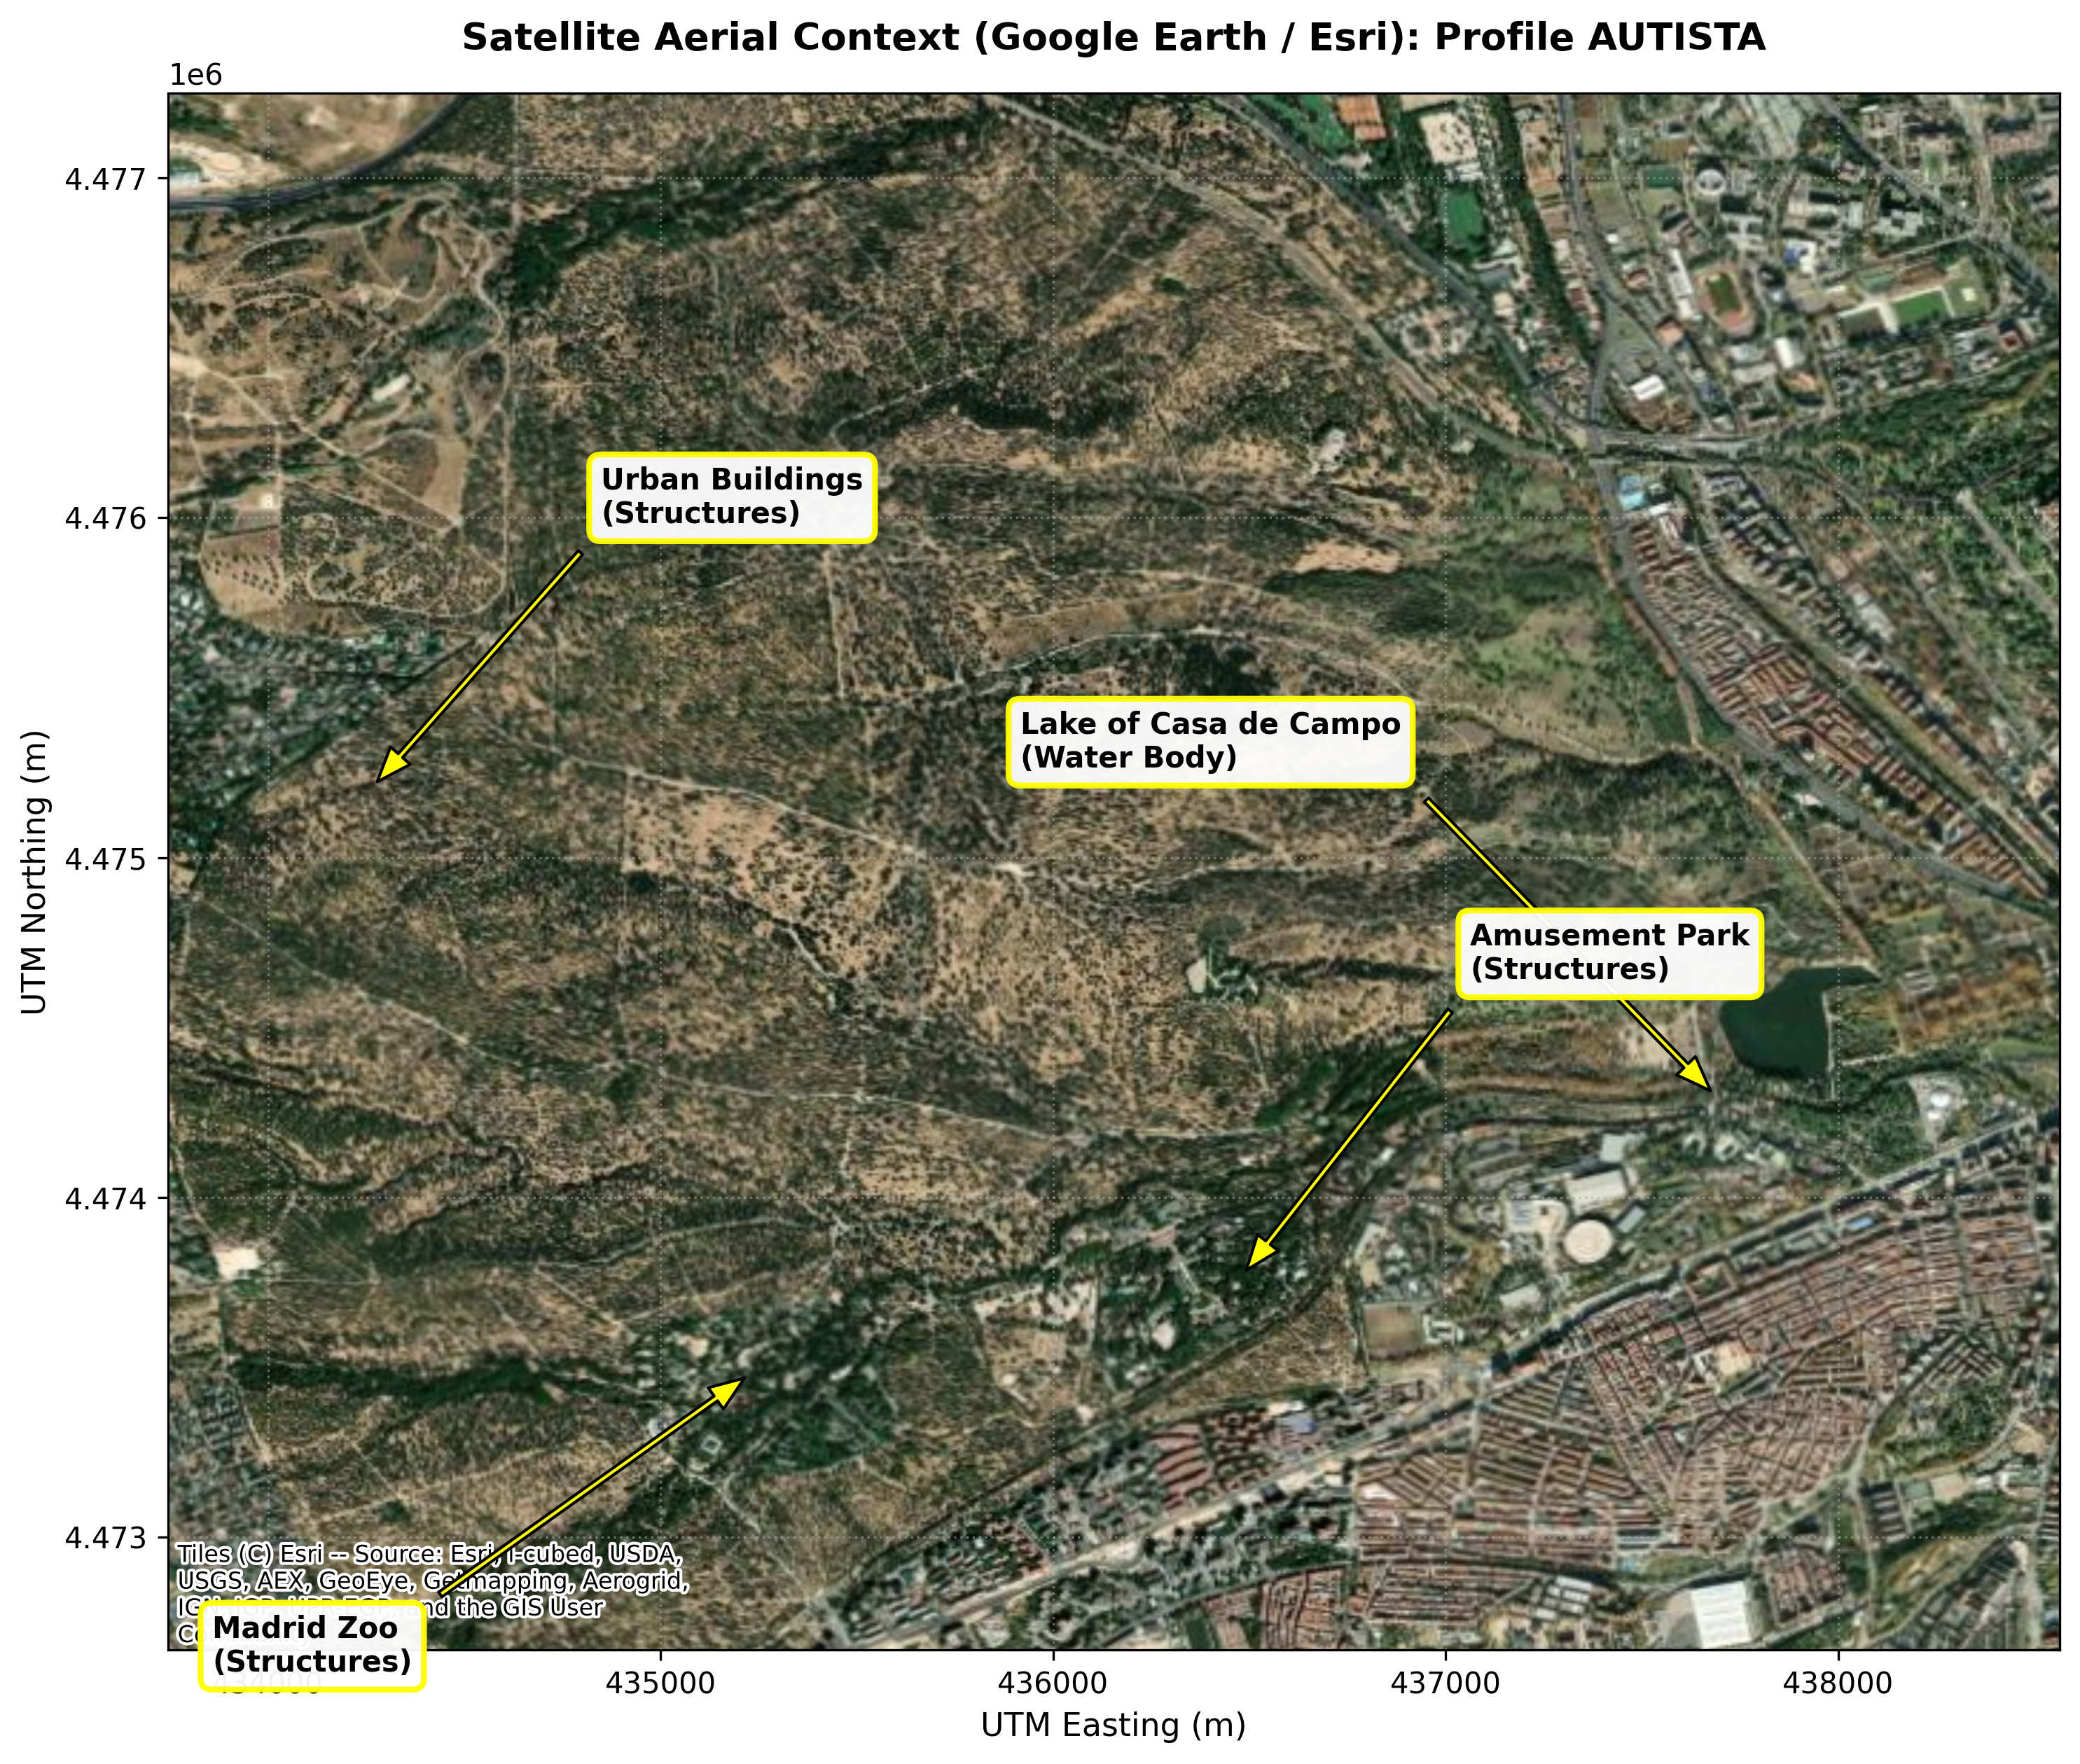
\includegraphics[width=0.95\textwidth]{imagenes/filtro_restricciones_satelite_autista.png}}
\end{figure}

\section{Observaciones y Modelo del Sensor (Sensor Ideal de Nivel 1)}

La capacidad del UAV para localizar a la víctima en el terreno se modela mediante el enfoque canónico de \textbf{Sensor Ideal de Huella Geométrica (Nivel 1)}, adaptado del modelo de observación desarrollado por Yago Brotón.

Bajo este modelo, la probabilidad de detección condicional $P_d(x,y \mid p_k)$ de una víctima ubicada en las coordenadas $(x,y)$ dada la posición del dron $p_k = (x_k, y_k)$ a una altitud de vuelo $h$ se define como una función determinista de cobertura binaria:
\begin{equation}
    P_d(x,y \mid p_k) = \begin{cases} 
        1.0 & \text{si } \sqrt{(x - x_k)^2 + (y - y_k)^2} \le R_d \\ 
        0.0 & \text{en otro caso} 
    \end{cases}
\end{equation}
donde $R_d$ representa el radio de cobertura efectiva de la cámara a bordo, el cual viene determinado por la altitud $h$ y el ángulo del campo de visión (\textit{Field of View - FoV}) $\theta_{\text{FoV}}$:
\begin{equation}
    R_d = h \cdot \tan\left(\frac{\theta_{\text{FoV}}}{2}\right)
\end{equation}

Para las condiciones nominales de vuelo en la Casa de Campo ($h = 50\text{ m}$ de altitud y $\theta_{\text{FoV}} = 90^\circ$), el radio de cobertura resultante en el suelo es exactamente $R_d = 50\text{ metros}$.

Dado el tamaño de celda de $10\text{ m} \times 10\text{ m}$, una huella circular de $R_d = 50\text{ m}$ cubre un radio discreto de 5 celdas a partir de la posición del dron. Si el centroide de una celda queda dentro de este radio de barrido, la celda se marca como observada y su probabilidad acumulada es absorbida por el dron.

\section{Filtro Recursivo Bayesiano (RBF) y Mapa de Creencias Residual}

Cuando un dron sobrevuela una región y no detecta a la víctima, esta observación negativa aporta información. El sistema debe reducir la probabilidad de presencia en las celdas observadas y, por conservación de la masa de probabilidad, aumentar proporcionalmente la probabilidad en el resto de las zonas no exploradas.

Este proceso de actualización dinámica de la matriz de creencias se implementa mediante el Filtro Recursivo Bayesiano. Denotemos como $b_t(i, j)$ la creencia (prior) de que la víctima está en la celda $(i, j)$ en el tiempo $t$. Si el dron inspecciona el área en el paso $t$ y la observación $y_t$ es negativa ($y_t = 0$, víctima no encontrada), la creencia actualizada para el paso $t+1$ se calcula aplicando el teorema de Bayes:
\begin{equation}
    b_{t+1}(i, j) = P\left(x = (i,j) \mid y_t = 0, b_t\right) = \frac{P\left(y_t = 0 \mid x = (i,j)\right) \cdot b_t(i, j)}{P\left(y_t = 0 \mid b_t\right)}
\end{equation}

Dado que bajo el sensor ideal $P\left(y_t = 1 \mid x = (i,j)\right) = P_d(i, j)$, la probabilidad de no detección condicional es $P\left(y_t = 0 \mid x = (i,j)\right) = 1 - P_d(i, j)$. La regla de actualización del RBF para cada celda $(i, j)$ es:
\begin{equation}
    b_{t+1}(i, j) = \frac{\left(1 - P_d(i, j)\right) \cdot b_t(i, j)}{1 - \sum_{u=1}^{N_y} \sum_{v=1}^{N_x} P_d(u, v) \cdot b_t(u, v)}
\end{equation}
Este filtro redistribuye dinámicamente la masa de probabilidad durante la simulación, guiando a los planificadores inteligentes hacia zonas no exploradas que aún conservan alta probabilidad de éxito.

\section{Simulación de Víctimas y Evaluación Estadística (Método de Montecarlo)}

Para validar la eficacia de los algoritmos de enrutamiento y estimar sus métricas de rendimiento reales, se requiere una validación matemática consistente. En el framework integrado, esto se implementa mediante simulaciones estadísticas de Montecarlo.

En un despliegue de rescate real, los drones buscan a \textbf{una única persona}. En la experimentación, simular $N = 50$ semillas independientes significa que el sistema ejecutará \textbf{50 misiones completas e independientes}:
\begin{itemize}
    \item \textbf{Punto Inicial Fijo de Despegue (LKP):} En todas las 50 ejecuciones, el dron despega de manera determinista desde el centro geométrico del parque o Punto de Planificación Inicial (LKP), reflejando el puesto de mando de emergencias.
    \item \textbf{Generación Estocástica de Víctimas:} En cada simulación $k \in \{1, \dots, 50\}$, el sistema genera de forma estocástica la ubicación de una sola víctima virtual $v_k$ en el mapa. Esta siembra se realiza mediante un muestreo ponderado sobre el mapa de calor $b(v^0)$ restringido a celdas transitables ($P > 0$).
    \item \textbf{Criterio de Descubrimiento:} Durante la simulación del universo $k$, se comprueba si la trayectoria del dron intercepta la huella del sensor de la víctima ($d \le 50\text{ m}$) en algún paso de tiempo. Si lo hace, la búsqueda se considera un \textbf{éxito} ($x_k = 1$). De lo contrario, es un fallo ($x_k = 0$).
\end{itemize}

\begin{figure}[H]
	\ffigbox[\FBwidth]
	{\caption{CROQUIS DE EVALUACIÓN MONTECARLO: DESPEGUE FIJO (LKP) Y MUESTREO DE VÍCTIMAS ESTOCÁSTICAS}}
	{\label{fig:croquis_montecarlo}
	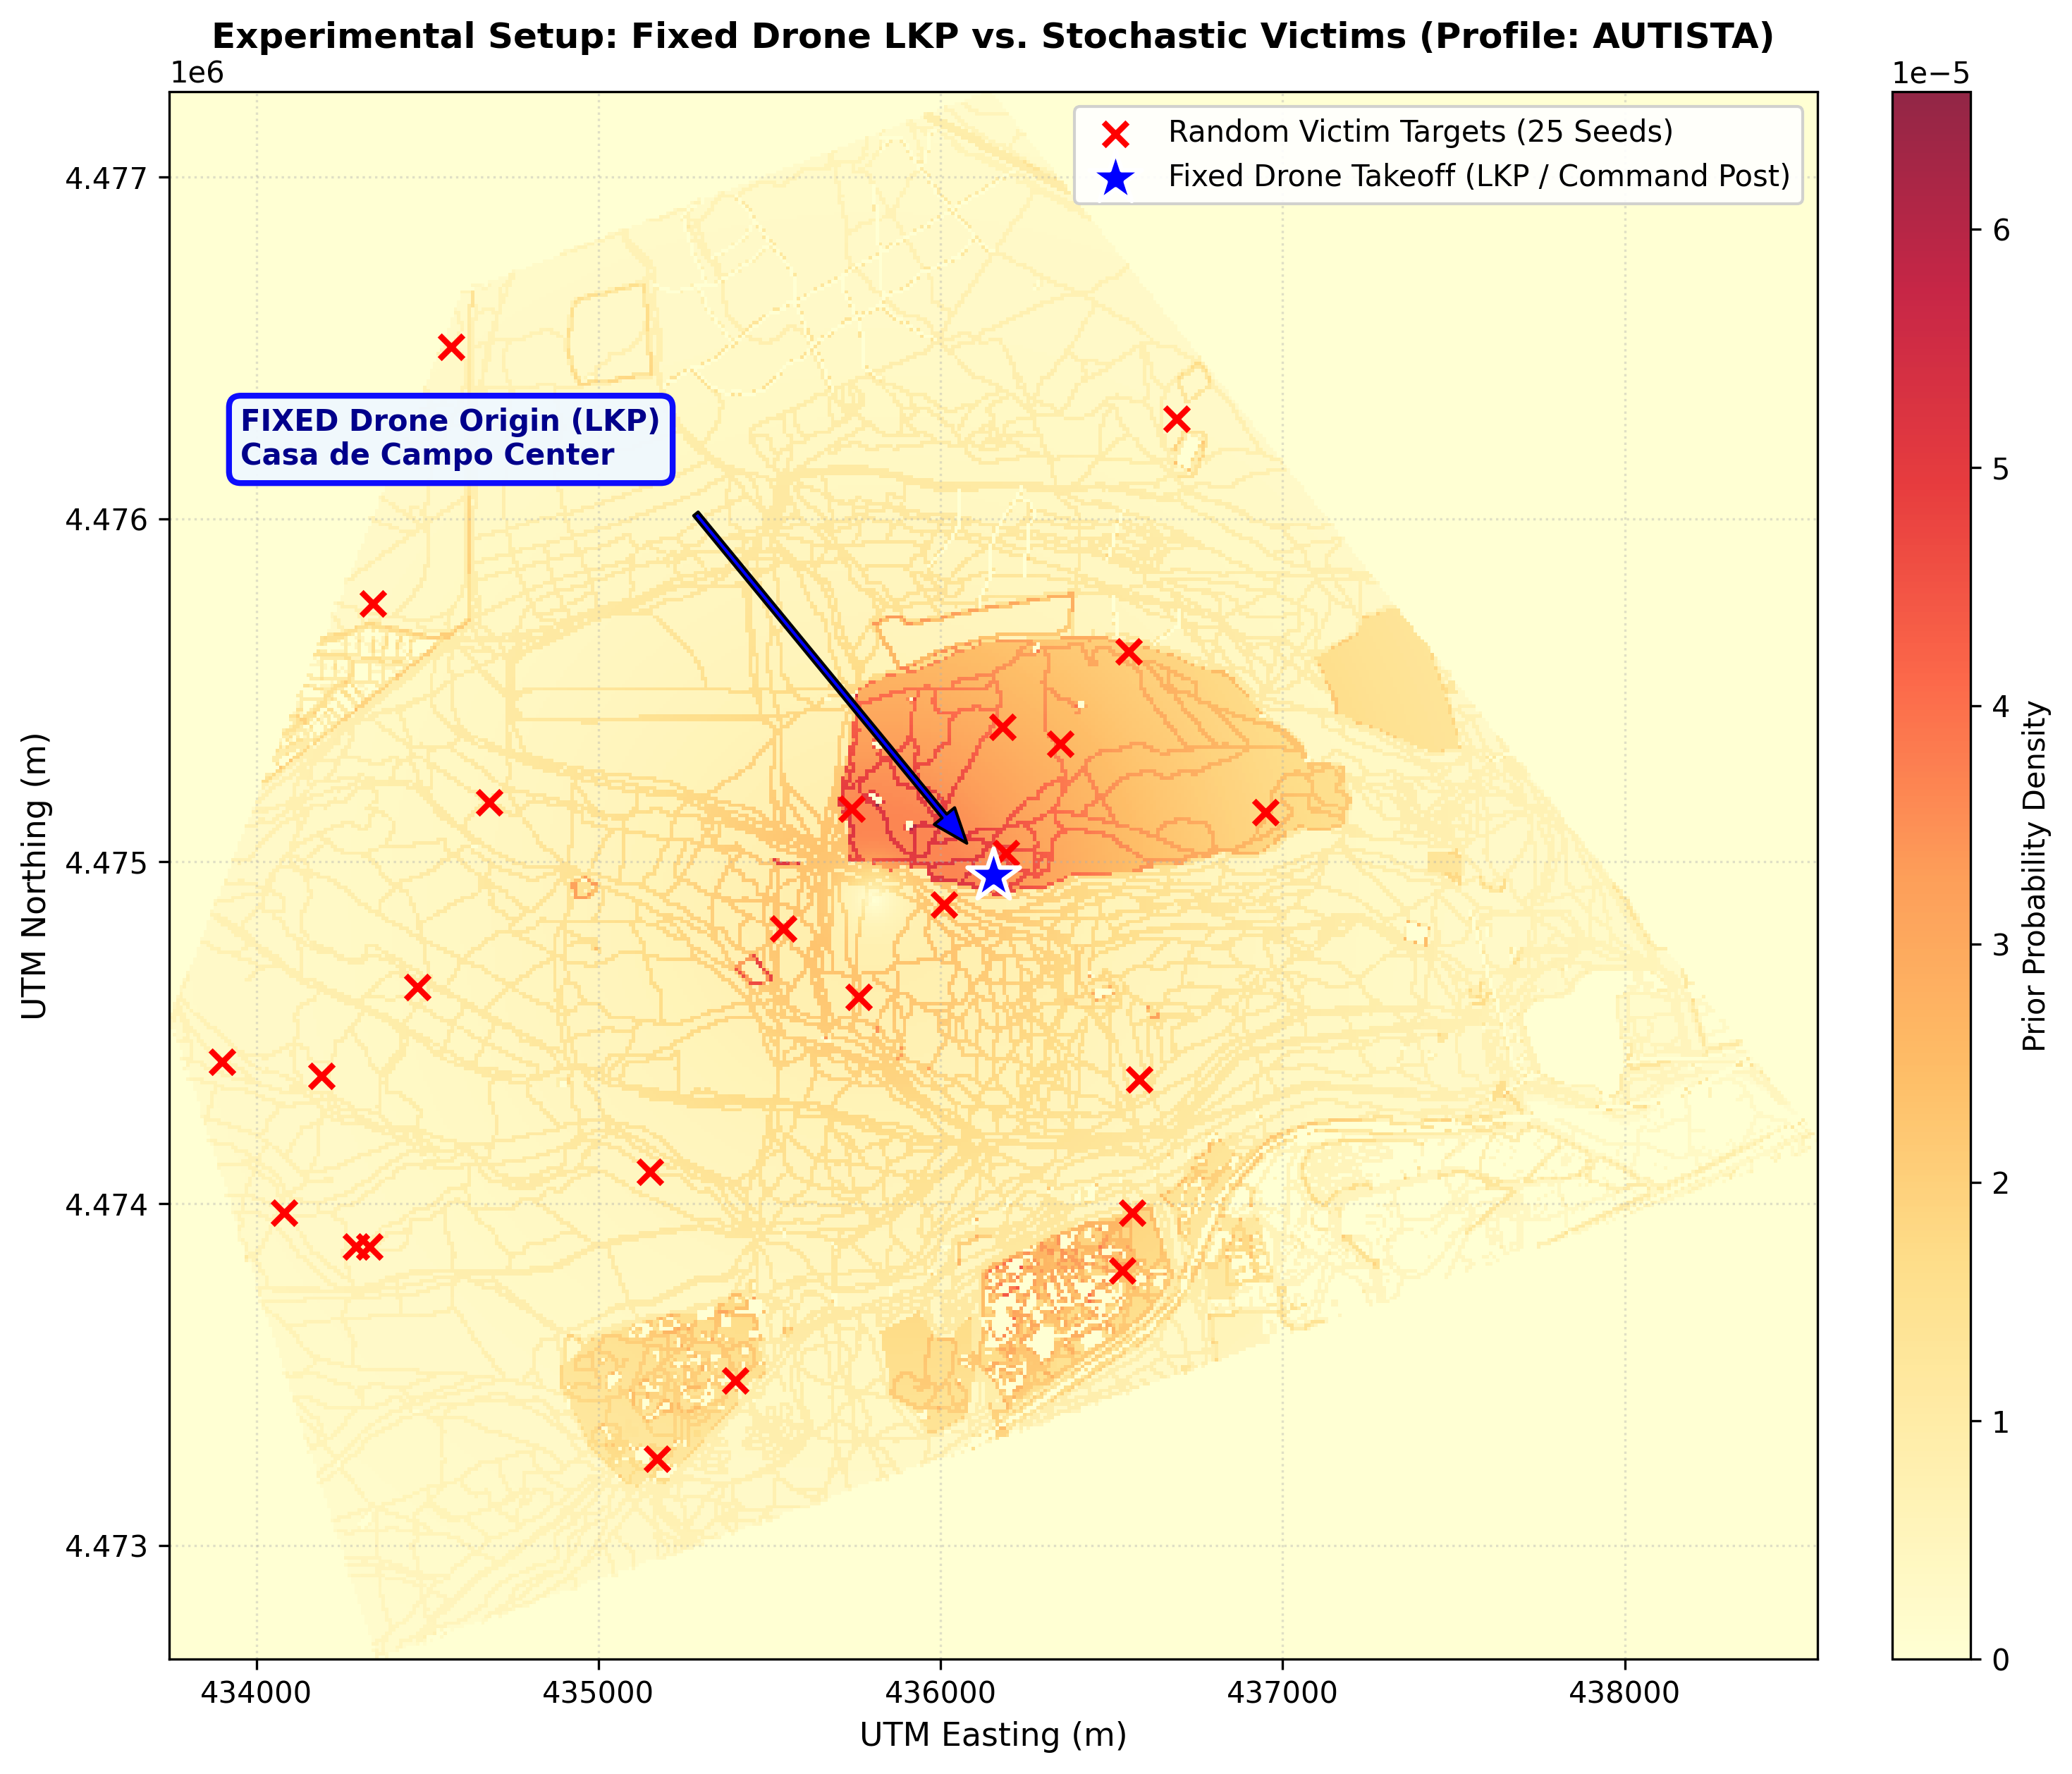
\includegraphics[width=0.90\textwidth]{imagenes/croquis_aleatoriedad_escenario.png}}
\end{figure}

El promedio de éxitos sobre las 50 simulaciones independientes define la métrica de éxito empírico:
\begin{equation}
    \text{Success Rate} = \frac{1}{N} \sum_{k=1}^{N} x_k
\end{equation}
Esta tasa acumulada proporciona robustez estadística, garantizando que el rendimiento reportado para un algoritmo no sea fruto de la suerte espacial de una única ejecución.
